\documentclass{beamer}
%%% ========== Package setup ==========
\usepackage{xeCJK}      % Chinese words package
\usepackage{fontspec}   % Word fonts package
\usepackage{listings}
\usepackage{wrapfig}
\usepackage{multicol}   % Multicolumn package

%%% ========== Slide setting ==========
%% Slide theme setup
\usetheme{Madrid}

%% Setup chinese words encoder
\XeTeXlinebreaklocale "zh"
\XeTeXlinebreakskip = 0pt plus 1pt

%% More word fonts
% \setmainfont{Times New Roman}
\renewcommand{\familydefault}{\rmdefault}
\setCJKmainfont{標楷體}

% Setting for figure and table numbering
\setbeamertemplate{caption}[numbered]

%%% ========== Title setup ==========
\date{January 25, 2022}
\title{Meeting}
\author{Po-Hsun Wu}

%%% ========== Document ==========
\begin{document}
    \frame{\titlepage}

    \section{Progress report}

    \begin{frame}
        \frametitle{\secname}
        \begin{itemize}
            \item Get the data from XPlane123
        \end{itemize}
        \begin{figure}
            \centering
            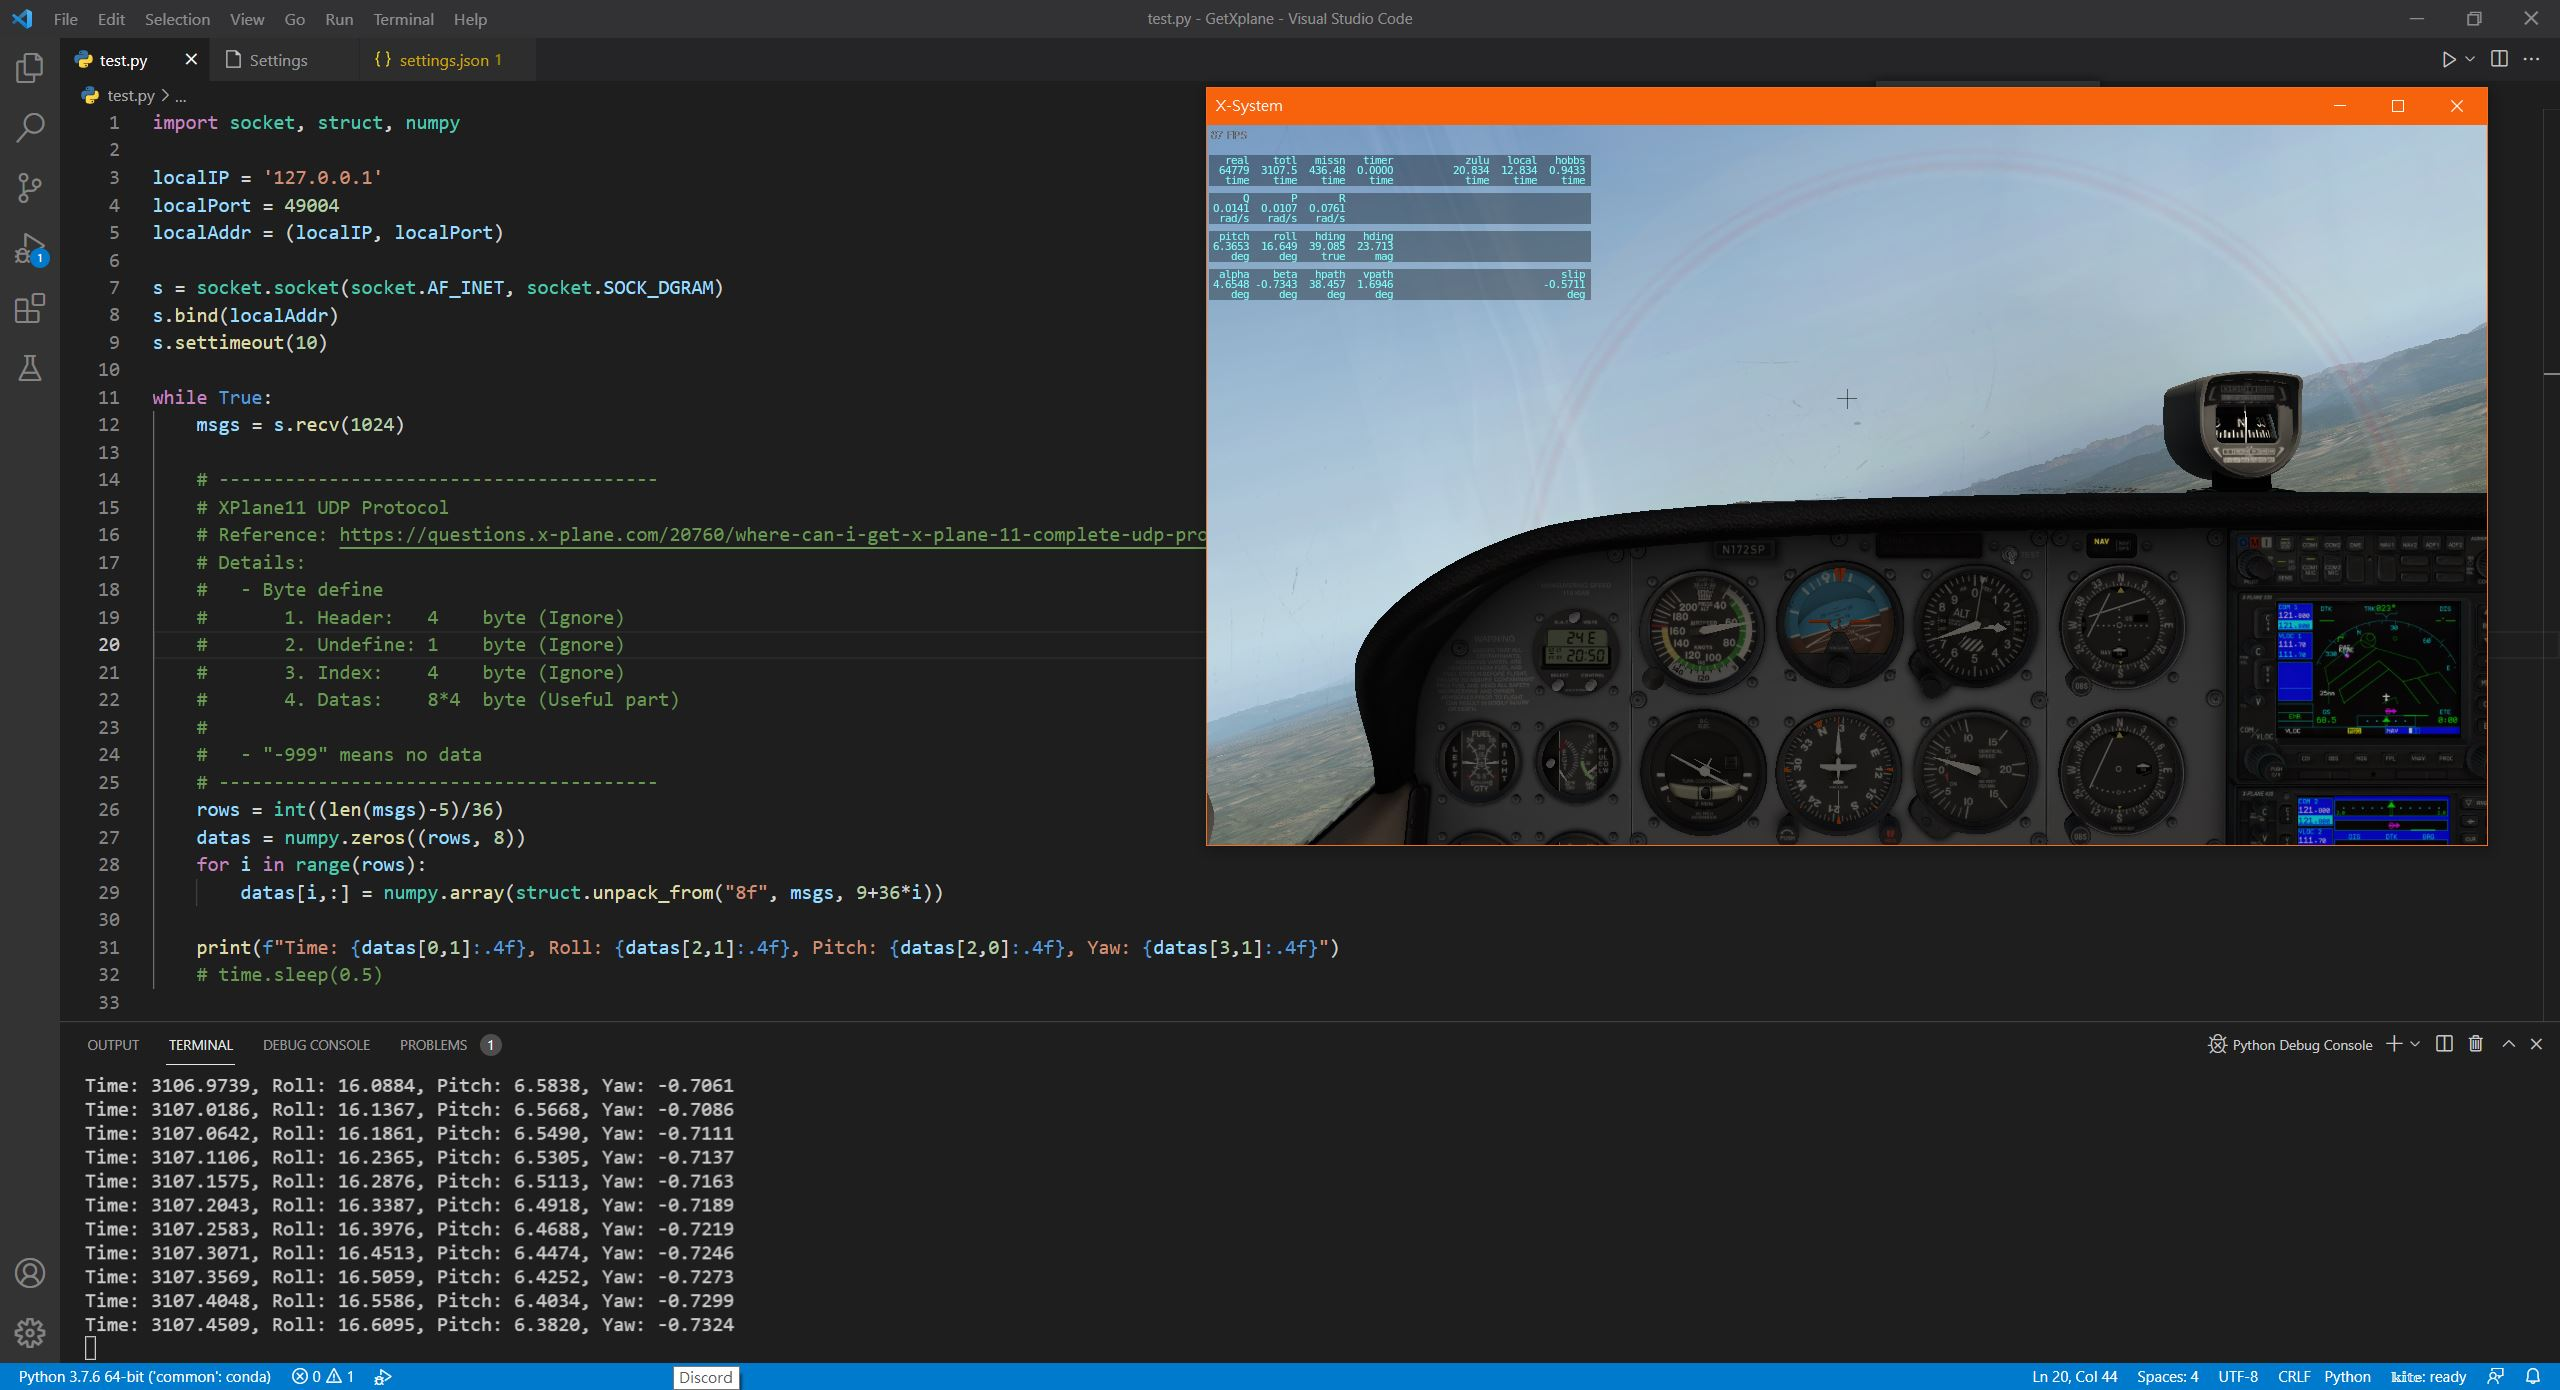
\includegraphics[scale=.2]{Figs/Result.JPG}
            \caption{Connect result}
        \end{figure}
    \end{frame}

    \section{Future}

    \begin{frame}
        \frametitle{\secname}
        \begin{itemize}
            \item Simplify the program.
            \item Review the basic knowledge for ML.
        \end{itemize}

    \end{frame}

\end{document}
